\documentclass[a4paper]{article}

\usepackage{amsthm}

\usepackage{tikz}

\newtheorem{example}{Example}[section]

\title{Nasty examples}

\author{Johannes Marti and Leif Sabellek}

\begin{document}

\maketitle

\section{Strange tree pattern}

\begin{example}
Colors $a$, $b$ and $c$ with $a \to b$, $b \to c$, $c \to a$ and $x \to
x$ for all $x \in \{a,b,c\}$.
\[
 \begin{array}{rcl}
 00000 & \mapsto & a \\
 00001 & \mapsto & b \\
 00010 & \mapsto & b \\
 00011 & \mapsto & c \\
 00100 & \mapsto & b \\
 00101 & \mapsto & c \\
 00110 & \mapsto & c \\
 00111 & \mapsto & a \\
 01000 & \mapsto & b \\
 01001 & \mapsto & c \\
 01010 & \mapsto & c \\
 01011 & \mapsto & a \\
 01100 & \mapsto & c \\
 01101 & \mapsto & a \\
 01110 & \mapsto & a \\
 01111 & \mapsto & b \\
\end{array}
\]
\end{example}


\section{All paths}

\begin{center}
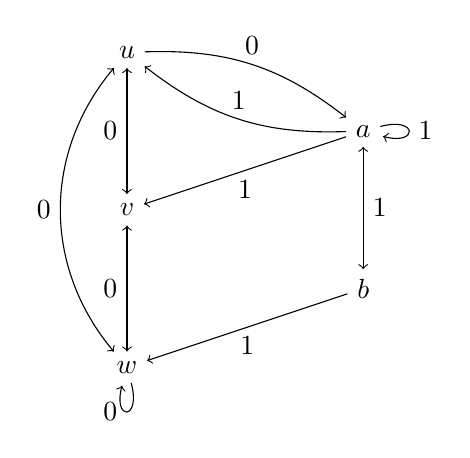
\begin{tikzpicture}
 \node (u) at (0,4) {$u$};
 \node (v) at (0,2)  {$v$};
 \node (w) at (0,0)  {$w$};

 \node (a) at (3,3) {$a$};
 \node (b) at (3,1) {$b$};

 \draw [<->] (u) edge node[left] {$0$} (v);
 \draw [<->] (v) edge node[left] {$0$} (w);
 \draw [<->] (u) edge [bend right=40] node[left] {$0$} (w);
 \draw [->] (w) edge [loop below] node[left] {$0$} (w);

 \draw [->] (u) edge [bend left=20] node [above] {$0$} (a);
 \draw [->] (a) edge [bend left=20] node [above] {$1$} (u);
 \draw [->] (a) edge node [below] {$1$} (v);

 \draw [->] (b) edge node [below] {$1$} (w);

 \draw [->] (a) edge [loop right] node [right] {$1$} (a);
 \draw [<->] (a) edge node [right] {$1$} (b);
\end{tikzpicture}
\end{center}
I think in this pattern nodes for all worlds exists. But the path from
$01 \dots$ to $0 \dots$ is of odd length. It should however be of even
lenght.



\end{document}
